\section{Interfaz gráfica y Jugabilidad}

El juego como ya se ha comentado consistirá en ver cómo los NPCs aplican una estrategia concreta, en este caso es el jugador el que a través de botones puede interaccionar para cambiar la estrategia. En la siguiente figura podemos ver cómo queda la interfaz.

\begin{figure}[H]
    \centering
    \newcommand{\behaviourmodes}{../IA_Juegos/Assets/Textures/UI}
\begin{tikzpicture}
    \sffamily\sansmath
    \node[draw, rounded corners, minimum width = 5cm, minimum height = 1cm, fill = white] (0) {TOTAL WAR};
    \node (1) [right = -1.3cm of 0] {
\includegraphics[scale=0.11]{\behaviourmodes/AttackMode}};
    \node (2) [left = -1.3cm of 0] {
\includegraphics[scale=0.11]{\behaviourmodes/AttackMode}};
    
    \node[draw, align = left, rounded corners, minimum width = 1.5cm, minimum height = 1cm, fill = white] (3) at (-1.1, -1.1) {\phantom{l}A\phantom{llllllllllll}};
    \node (4) [right = -1.3cm of 3] {
\includegraphics[scale=0.11]{\behaviourmodes/AttackMode}};
    
    \node[draw, align = left, rounded corners, minimum width = 1.5cm, minimum height = 1cm, fill = white] (5) at (1.1, -1.1) {\phantom{l}A\phantom{llllllllllll}};
    \node (6) [right = -1.3cm of 5] {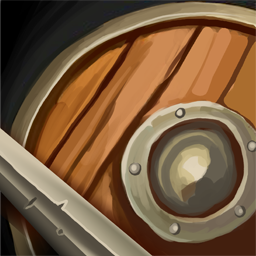
\includegraphics[scale=0.11]{\behaviourmodes/DefenseMode}};
    
    \node[draw, align = left, rounded corners, minimum width = 1.5cm, minimum height = 1cm, fill = white] (7) at (-1.1, -2.2) {\phantom{l}B\phantom{llllllllllll}};
    \node (8) [right = -1.3cm of 7] {
\includegraphics[scale=0.11]{\behaviourmodes/AttackMode}};
    
    \node[draw, align = left, rounded corners, minimum width = 1.5cm, minimum height = 1cm, fill = white] (9) at (1.1, -2.2) {\phantom{l}B\phantom{llllllllllll}};
    \node (10) [right = -1.3cm of 9] {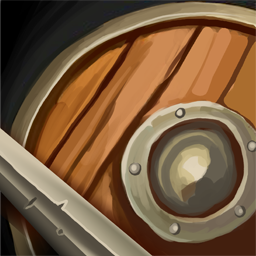
\includegraphics[scale=0.11]{\behaviourmodes/DefenseMode}};
\end{tikzpicture}
    \caption{Interfaz gráfica estrategia}
    \label{fig:mainButtons}
\end{figure}

Los iconos de espadas permitirán poner el modo ofensivo al equipo que se desee mientras que el icono del escudo permite indicar al equipo que se ponga a defender. El botón de \textit{Total War} cambia el comportamiento de todas las unidades del juego para que estas den prioridad al enfrentamiento y toma de la base rival. El juego comenzará con los botones desactivados.

Además tendremos una segunda UI a la que accederemos presionando la tecla \keys{I}. Esta nos permitirá tener el mapa de influencias en grande y el mapa de juego normal en un mini mapa, teniendo la siguiente interfaz que permite cambiar el mapa que se muestra.

\begin{figure}[H]
    \centering
    \begin{tikzpicture}
        \sffamily\sansmath
        \node[draw, rounded corners, minimum width = 5cm, minimum height = 1cm, fill = white] (0) {CAMBIAR MAPA};
        \node (1) [above = 0cm of 0] {MAPA ACTUAL: Tensión};
    \end{tikzpicture}
    \caption{Interfaz gráfica cambio de mapa}
    \label{fig:mainButtons}
\end{figure}

Por otra parte, se puede activar una opción para mostrar la acción que está realizando cada personaje de forma visual en el juego. Esta opción se activa presionando la tecla \keys{E}.

\begin{figure}[H]
    \centering
    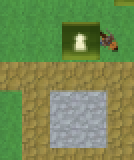
\includegraphics{images/actionState.png}
    \caption{Acción del personaje}
    \label{fig:actionState}
\end{figure}

\clearpage
A continuación mostramos una tabla con las distintas imágenes asociadas a cada estado.

\begin{table}[H]
    \centering
    \newcommand{\ActionStatesPath}{../IA_Juegos/Assets/Textures/UI/Resources}
    \resizebox{0.6\textwidth}{!}{
    \begin{tabular}{|>{\centering\arraybackslash}m{0.3\textwidth}|>{\centering\arraybackslash}m{0.3\textwidth}|}
        \hline
        Imagen & Acción asociada \\
        \hline
        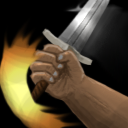
\includegraphics[scale=0.4]{\ActionStatesPath/AttackEnemy} & Atacar enemigo \\
        \hline
        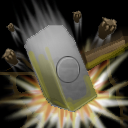
\includegraphics[scale=0.4]{\ActionStatesPath/CaptureBase} & Capturar la base enemiga \\
        \hline
        
\includegraphics[scale=0.4]{\ActionStatesPath/Defend} & Defender base propia \\
        \hline
        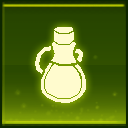
\includegraphics[scale=0.4]{\ActionStatesPath/GoHealing} & Ir a curarse \\
        \hline
        
\includegraphics[scale=0.4]{\ActionStatesPath/GoToEnemyBase} & Ir a la base enemiga \\
        \hline
        
\includegraphics[scale=0.4]{\ActionStatesPath/Heal} & Curarse \\
        \hline
    \end{tabular}
    }
    \caption{Leyenda de acciones}
    \label{tab:actionStates}
\end{table}

Esto se ha implementado mediante la clase \texttt{FollowStates}. Esta clase tiene referencias tanto del personaje como de una imagen próxima a él. Se ha definido también un enumerado, llamado \texttt{ActionState} que recoge cada una de las acciones vistas en la tabla anterior. Cada agente posee una variable de tipo este enumerado y es la que nos servirá para llevar a cabo esta labor.

\lstinputlisting[linerange=8-16, firstnumber=8]{\ScriptsPath/FollowStates.cs}

En cada frame se asigna la nueva posición en función del agente y se le asigna la imagen que le corresponda. 

\lstinputlisting[linerange=42-43, firstnumber=42]{\ScriptsPath/FollowStates.cs}
